Once the wafer has been fabricated, the values of $\u$ are fixed at all locations on the wafer; however, this distribution remains unknown for us.
In order to infer it, we employ the procedure, referred to as the statistical model, described in the current subsection and displayed in \fref{inference}.
The development of the statistical model closely follows \sref{preliminaries} and consists of the five components described below.

\subsubsection{Model of the \qoi}
The first step is to assign an adequate model to the unknown $\u$.
We model $\u$ as a Gaussian process \cite{rasmussen2006} since: (a) it is flexible in capturing the correlation patterns induced by the manufacturing process, and (b) it is computationally efficient; and (c) Gaussian distributions are often natural and accurate models for uncertainties due to process variation \cite{srivastava2010, juan2012}. Thus, we have
\begin{equation} \elabel{u-prior}
  \u | \vparam_\u \sim \gaussianp{\fMean}{\fCov}
\end{equation}
where $\fMean$ and $\fCov$ are the mean and covariance functions of $\u$, respectively.
Hereafter, the vertical bar, pronounced as ``given'', is used to mark the parameters that the probability distribution on the right-hand side depends on. In this case, such parameters are $\vparam_\u$, which we shall identify later on.
Prior to taking any measurements, $\u$ is assumed to be spatially unbiased; therefore, we let $\fMean$ be a single location-independent parameter $\mu_\u$, \ie, $\fMean{r} = \mu_\u$, $\forall \r \in \domain$.
The covariance function $\fCov$ is chosen to be the following composition:
\begin{equation} \elabel{covariance-function}
  \fCov{\r, \r'} = \sigma_\u^2 \big( \eta \; \fCov_\SE(\r, \r') + (1 - \eta) \fCov_\OU(\r, \r') \big)
\end{equation}
where
\[
  \fCov_\SE(\r, \r') = e^{-\frac{\norm{\r - \r'}^2}{\ell_\SE^2}} \hspace{1em} \text{ and } \hspace{1em}
  \fCov_\OU(\r, \r') = e^{- \frac{\abs{\,\norm{\r} - \norm{\r'}\,}}{\ell_\OU}}
\]
are the squared exponential and Ornstein-Uhlenbeck correlation functions, respectively; $\sigma_\u^2$ represents the variance of $\u$; $\eta \in [0, 1]$ is a weighting coefficient; $\ell_\SE$ and $\ell_\OU > 0$ are so-called length-scale parameters; and $\norm{\cdot}$ stands for the Euclidean distance.
The choice of the covariance function $\fCov$ is guided by the observations of the correlation structures induced by the fabrication process \cite{chandrakasan2001, cheng2011}: $\fCov_\SE$ imposes similarities between the points on the wafer that are close to each other, and $\fCov_\OU$ imposes similarities between the points that are at the same distance from the center of the wafer.
$\ell_\SE$ and $\ell_\OU$ control the extend of these similarities, \ie, the range wherein the influence of one point on another is significant.
Although all the above parameters of the model of $\u$ can be inferred from the data, for simplicity, we shall focus on $\mu_u$ and $\sigma_\u^2$.
The rest of the parameters, namely, $\eta$, $\ell_\SE$, and $\ell_\OU$ of the covariance function $\fCov$, are assumed to be determined prior to our analysis based on the knowledge of the correlation patterns typical for the production process utilized (see \cite{marzouk2009} and references therein).
At this point, we have established a model for $\u$; however, due to the infinite dimensionality, it is computationally intractable, which we address next.

\begin{figure}
  \centering
  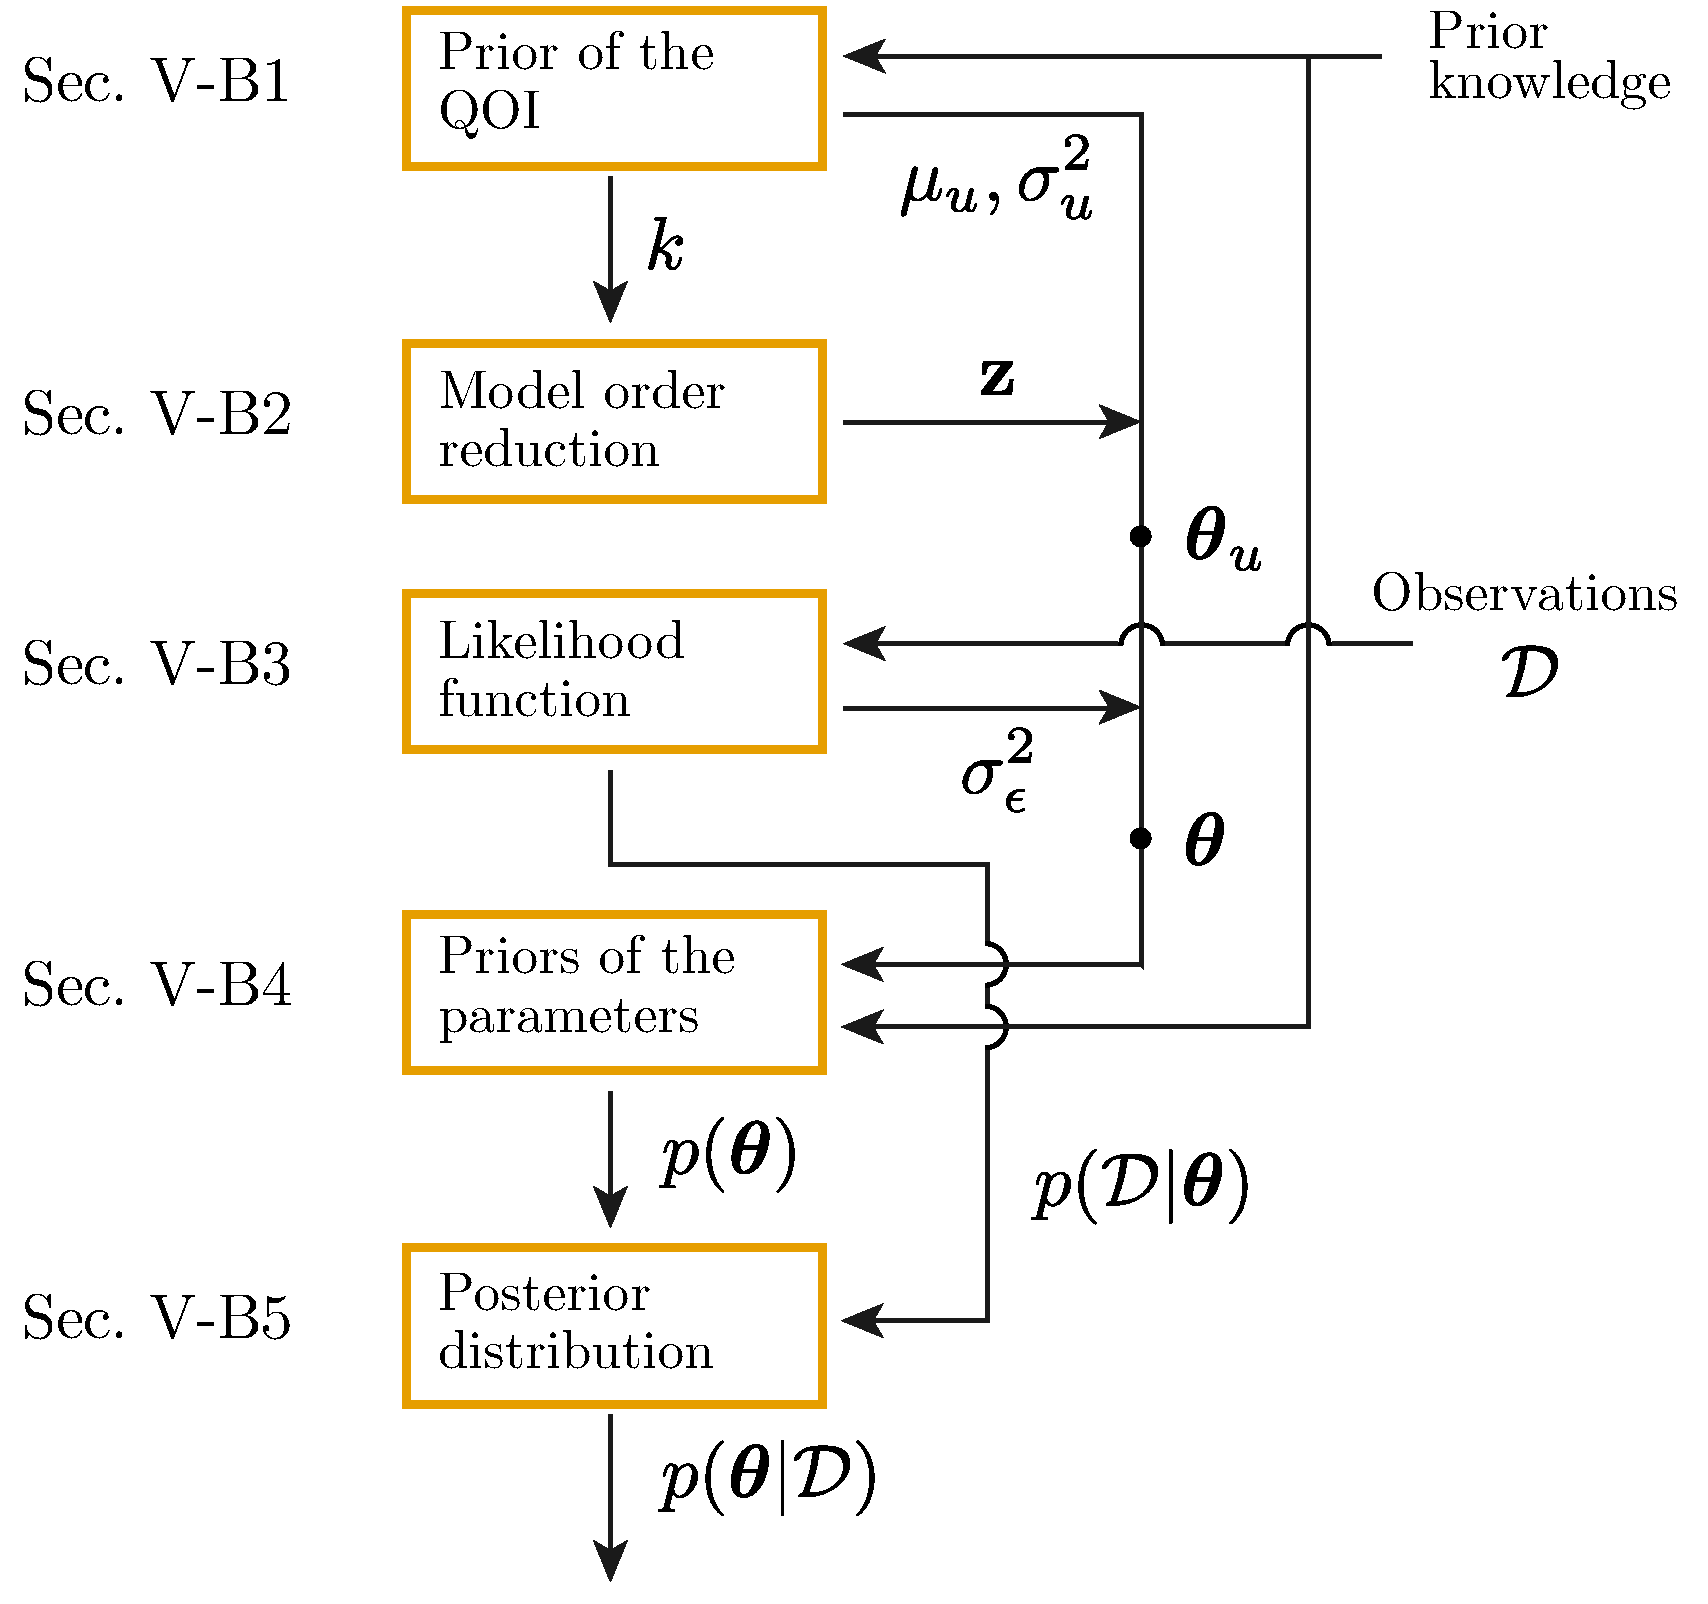
\includegraphics[width=1.0\linewidth]{include/figures/inference.pdf}
  \vspace{-0.7em}
  \caption{The statistical model.}
  \flabel{inference}
  \vspace{-1.3em}
\end{figure}

\subsubsection{Model order reduction} \slabel{model-order-reduction}
The random element $\u$ is an infinite-dimensional object as it characterizes a continuum of spatial locations.
For practical computations, however, it should be reduced to a finite-dimensional one.
First, $\u$ is discretized with respect to the union of two sets of points on the wafer: the first one is composed of the $\nrdies \nrprocs$ points where the observations in $\QData$ were made (one location for each measured processing element on each measured die), and the other of the points where the user wishes to characterize $\u$.
For simplicity, we assume that the user is interested in all processing elements at all measurement sites, which is $\ndies \nprocs$ locations in total (see \fref{wafer-measured}). Consequently, we obtain an $\ndies \nprocs$-dimensional representation of $\u$ denoted by the vector $\vu$.
Second, the dimensionality of the \qoi\ is reduced even further by applying the well-known principal component analysis to the covariance matrix of $\vu$ computed via \eref{covariance-function}.
More precisely, we factorize the computed matrix using the eigenvalue decomposition \cite{press2007} and discard those eigenvalues (and their eigenvectors) whose contribution to the total sum of the eigenvalues is below a certain threshold.
The result is
\begin{equation} \elabel{kl-approximation}
  \vu = \mu_\u \vI + \sigma_\u \mKL \vz
\end{equation}
where $\vI = (e_i = 1) \in \real^{\ndies \nprocs}$, $\mKL \in \real^{\ndies \nprocs \times \nvars}$, and $\vz = (\z_i) \in \real^\nvars$ obey the standard Gaussian distribution.
$\nvars$ is the final dimensionality of the model of $\u$; typically, $\nvars \ll \ndies \nprocs$.
Consequently, the \qoi\ is now ready for practical computations.
In what follows, the parameters of \eref{u-prior} are defined by $\vparam_\u = \{ \vz, \mu_\u, \sigma^2_\u \}$ (see \fref{inference}).

\subsubsection{Likelihood function}
In the Bayesian context, the observed information is taken into account via a likelihood function (see \sref{preliminaries}).
In our case, this information is the measurements $\QData$ stacked into $\vq^\meas$ as described in \sref{data-model}.
Since the measurement process is not perfect, we should also take into consideration the measurement noise.
To this end, for a given $\u$, the observed $\vq^\meas$ is assumed to deviate from the data model prediction $\vq$ as follows:
\begin{equation} \elabel{noisy-measurements}
  \vq^\meas = \vq + \vnoise
\end{equation}
where $\vnoise$ is an $\nrdies \nrprocs \nrsteps$-dimensional vector of noise, which is typically assumed to be a white Gaussian noise \cite{rasmussen2006, marzouk2009}.
Without loss of generality, the noise is assumed to be independent of $\u$ and to have the same magnitude for all measurements (characterized by the utilized instruments).
Consequently, the model of the noise is
\begin{equation} \elabel{noise-model}
  \vnoise | \sigma^2_\noise \sim \gaussian{\vZero}{\sigma^2_\noise \mOne}
\end{equation}
where $\sigma^2_\noise$ is the variance of the noise, and $\mOne$ is the identity matrix.
Let us denote the parameters of the inference by $\vparam = \vparam_\u \cup \{ \sigma_\noise^2 \} = \{ \vz, \mu_\u, \sigma_\u^2, \sigma_\noise^2 \}$ (observe this union in \fref{inference}).
Finally, combining \eref{noisy-measurements} and \eref{noise-model}, we obtain
\begin{equation} \elabel{likelihood}
  \vq^\meas | \vparam \sim \gaussian{\vq}{\sigma_\noise^2 \mOne}.
\end{equation}
The probability density function of this distribution is the likelihood function $\f{\QData | \vparam}$ of our statistical model, which is the first of the two components needed for the posterior given in \eref{bayes}.

\subsubsection{Priors of the parameters}
The second component of the posterior in \eref{bayes} is the prior $\f{\vparam}$, which we now need to decide on. In this paper, we put the following priors on $\vparam$:
\begin{align}
  & \vz \sim \gaussian{\vZero}{\mOne}, \hspace{1em} \mu_\u \sim \gaussian{\mu_0}{\sigma^2_0}, \elabel{priors} \\
  & \sigma^2_\u \sim \sichisquared{\nu_\u}{\tau^2_\u}, \text{ and } \sigma^2_\noise \sim \sichisquared{\nu_\noise}{\tau^2_\noise}. \nonumber
\end{align}
The prior for $\vz$ is due to the properties the decomposition in \eref{kl-approximation}.
The next three priors, \ie, a Gaussian and two scaled inverse chi-squared distributions, are a common choice for a Gaussian model with the mean and variance being unknown.
The parameters $\mu_0$, $\tau^2_\u$, and $\tau^2_\noise$ represent the presumable values of $\mu_u$, $\sigma^2_\u$, and $\sigma^2_\noise$, respectively, and are set by the user based on the prior knowledge on the technological process and measurement instruments employed. The parameters $\sigma_0$, $\nu_\u$, and $\nu_\noise$ reflect the precision of this prior information.
When the prior knowledge is weak, non-informative priors can be utilized \cite{gelman2004}.
Taking the product of the densities in \eref{priors}, we obtain the prior $\f{\vparam}$ completing \eref{bayes}.

\subsubsection{Posterior}
At this point, we have obtained the two pieces of the posterior shown in \eref{bayes}: the likelihood function, which is the density in \eref{likelihood}, and the prior, which is the product of the four densities in \eref{priors}. Thus, the posterior is
\begin{equation} \elabel{posterior}
  \f{\vparam | \QData} \propto \f{\vq^\meas | \vz, \mu_\u, \sigma^2_\u, \sigma^2_\noise} \; \f{\vz} \; \f{\mu_\u} \; \f{\sigma^2_\u} \; \f{\sigma^2_\noise}.
\end{equation}
Provided that we have a way of drawing samples from \eref{posterior}, the \qoi\ can be readily analyzed as we shall see in \sref{post-processing}.
The problem, however, is that the direct sampling of the posterior is not possible due to the data model involved in the likelihood function via $\vq$ (see \eref{likelihood} and \sref{data-model}).
In order to circumvent this problem, we utilize the Metropolis-Hastings (MH) algorithm \cite{gelman2004} introduced in \sref{preliminaries}.
The algorithm operates on an auxiliary distribution called the proposal distribution, which is chosen to be convenient for sampling.
Each sample, drawn from this proposal, is then used in \eref{posterior} to evaluate the posterior probability of this sample and decide whether it should be accepted or rejected.\footnote{A reject means that the sequence of samples advances using the last accepted sample; therefore, the chain of samples is never interrupted.}
The acceptance/rejection strategy of the MH algorithm pushes the produced chain of samples towards regions of high posterior probability, which, after a sufficient number of steps depending on the starting point of the chain and the efficiency of the moves, results in a good approximation of the target posterior distribution in \eref{posterior}.
The preliminary computations needed for the proposal construction are discussed next, and the further sampling procedure in \sref{sampling}.
